\documentclass[a4paper,10pt]{article}
\usepackage[utf8]{inputenc}
\usepackage{CJK, CJKnumb}
\usepackage{amsmath,amsfonts,amsthm,amssymb}
\usepackage{setspace}
\usepackage{fancyhdr}
\usepackage{lastpage}
\usepackage{extramarks}
\usepackage{chngpage}
\usepackage{soul,color}
\usepackage{xcolor}
\usepackage{graphicx,float,wrapfig}
\usepackage{subfigure}
\usepackage{listings}
\usepackage{enumerate}
\usepackage{multirow}
\usepackage{pxfonts}
\usepackage{cite}
\usepackage{url}

\renewcommand{\today}{\number\year 年 \number\month 月 \number\day 日}

\topmargin=-0.45in      %
\evensidemargin=0in     %
\oddsidemargin=0in      %
\textwidth=6.5in        %
\textheight=9.0in       %
\headsep=0.25in         %

\begin{document}

\lstset{numbers = left,
numberstyle = \tiny,
frame = shadowbox,
rulesepcolor = \color{red!20!green!20!blue!20},
tabsize = 4,
language=Java,
basicstyle=\tt
}
\begin{CJK*}{UTF8}{gbsn}
%opening
\CJKtilde
\title{Indoor Localization设计报告}
\author{胡威 2012012430,李竺霖2012011419,孔令航 2012011340}
\date{}
\maketitle

\section{程序功能}
Indoor Localization是一个Android平台上的手机应用,利用Wifi信号强度实现了室内定位功能。

\begin{enumerate}
 \item 查询位置时,只需要点击“LOCATE”按钮,应用就会开始扫描当前位置的Wifi信号,然后将数据上传到服务器。服务器会返回预测到的房间号,以文本形式展示在屏幕上。
 同时在地图上会显示服务器返回的位置信息和用户当前面向的方向。整个过程大约需要3到4秒时间,过程中会有进度条指示进度,并且也会以文字形式说明“Scanning Wifi”或“Wifi scanned,now locating”。
 如果网络出现错误则提示“Fail to connect”。
 \item 上传位置时,需要输入房间号和当前的X、Y坐标,然后点击“UPLOAD”,应用会在当前位置扫描5组数据,取平均后上传到服务器。整个过程持续20秒左右,有进度条标示进度,并且也会以文本形式
 说明当前已经扫描完多少组数据。
 \item 应用在启动时会显示一个启动画面,之后进入主界面。在主界面中可以通过点击“LOCATE”和“UPLOAD”两个标签(不是前面所说的按钮,见下面示意图)或者滑动屏幕来切换功能。标签下方有一个色带,可以标示当前所在
 的功能页面。页面切换时滑动条会以动画的形式滑动到对应的新标签。
\end{enumerate}

本应用的运行界面如下:

\begin{figure}[h]
\begin{minipage}[t]{0.3\linewidth}
\centering
\includegraphics[width=1in]{1.jpg}
%\caption{Map}
%\label{map}
\end{minipage}
\begin{minipage}[t]{0.3\linewidth}
\centering
\includegraphics[width=1in]{2.jpg}
%\caption{SVR}
%\label{SVR}
\end{minipage}
\begin{minipage}[t]{0.3\linewidth}
\centering
\includegraphics[width=1in]{3.jpg}
%\caption{WKNN}
%\label{WKNN}
\end{minipage}
\end{figure}

\begin{figure}
\begin{minipage}[t]{0.3\linewidth}
\centering
\includegraphics[width=1in]{4.jpg}
%\caption{KNN}
%\label{KNN}
\end{minipage}
\begin{minipage}[t]{0.3\linewidth}
\centering
\includegraphics[width=1in]{5.jpg}
%\caption{KNN}
%\label{KNN}
\end{minipage}
\begin{minipage}[t]{0.3\linewidth}
\centering
\includegraphics[width=1in]{6.jpg}
%\caption{KNN}
%\label{KNN}
\end{minipage}
\end{figure}


\section{定位算法}

本应用采用室内定位常用的基于Wifi强度的方法\cite{1}。移动终端需要能够扫描到其所在位置附近的Wifi名称、强度等信息,Android 系统提供的接口可以很方便地实现这一功能。终端扫描到的所有Wifi信号有一个RSSI(Radio Signal Strength Indications)值表示它的强度,我们使用这些RSSI组成的向量作为这个位置的特征。定位算法建立在实验数据基础上,它分为两个阶段:
\begin{enumerate}[1)]
\item 离线(训练)阶段:在这一阶段我们测量多个位置的RSSI向量,并与它们的位置信息一起保存在数据库中。
\item 在线阶段:在这一阶段中移动终端扫描当前的Wifi信息,通过其RSSI向量与数据库中已保存信息的比对推测出当前的位置。具体算法请见后文。
\end{enumerate}

假设在离线阶段共测了$l$个点,其中第$i$个点的RSSI向量是$x_i \in \mathbb R^n$,位置是$y_i \in \mathbb R^d$,这里$n$是不同Wifi信号的个数,$d$是我们考虑的物理空间的维数。如果我们只考虑分类问题(如只需确定点在哪个房间),则可认为$d = 1$,$y_i$是类型的一个id(如房间号)。考虑一个在在线阶段测得的RSSI向量$x\in \mathbb R^n$,为推测它的位置$y$我们采用了WKNN和SVM-Regression两类算法,其中SVM的实现使用了libSVM包\cite{2}。对于分类问题我们还可以使用SVM-Classification算法计算。

\subsection{Weighted $k$ Nearest Neighbours (WKNN)}
设$k\le l$是一个固定的正整数,一个简单的算法是在训练集$\{x_i | 1 \le i \le l\}$中找与$x$距离(例如欧几里得距离)最近的$k$个点$x_{i_1}, \cdots, x_{i_k}$,然后对这$k$个点的位置取一个加权平均作为预测的位置:
\[
y = \frac{\sum\limits_{j=1}^k \frac{y_{i_j}}{d(x, x_{i_j}) + d_0} }{\sum\limits_{j=1}^k \frac{1}{d(x, x_{i_j}) + d_0} }
\]
其中$d(x, x_{i_j})$是两个$n$维向量的距离(例如欧几里得距离),$d_0$是一个很小的正常数以防出现分母为0的情况。

一个更简单的算法是KNN,也就是$k$ Nearest Neighbours。顾名思义,它直接对$k$个点取(不加权)平均值。


\subsection{Support Vector Machines(SVM)}

SVM是机器学习中分类和回归问题非常有效的解法。我们对它做简单的介绍,更详细的介绍请参见\cite{3}。

\subsubsection{线性可分离问题}
先考虑最简单的二类分类问题,即$y_i \in \{-1, 1\}$。假如存在$n$维空间中的一个超平面$w^Tx+b = 0$将两类点分开,如图\eqref{SVM-linear-separable-fig}。
\begin{figure}[htbp]
\centering
\includegraphics[width=7cm]{SVM1.png}
     \caption{Linear separable}
   \label{SVM-linear-separable-fig}
\end{figure}

SVM在满足这个要求的超平面中选出到最近数据点距离最远的一个,这等价于下面的二次规划问题:
\begin{equation}\label{SVM-linear-separable-opt}
\begin{aligned}
\text{minimize} \quad & \| w\|\\
\text{subject to} \quad & y_i(w^T x_i + b) \ge 1
\end{aligned}
\end{equation}

问题\eqref{SVM-linear-separable-opt}的对偶问题是:
\begin{equation}\label{SVM-linear-separable-dual-opt}
\begin{aligned}
\text{maximize} \quad & \sum_{i=1}^l \lambda_i - \frac{1}{2} \sum_{i=1}^l \sum_{j=1}^l \lambda_i\lambda_jy_iy_jx_i^Tx_j^T\\
\text{subject to} \quad & \sum_{i=1}^l \lambda_iy_i =0\\
& \lambda_i \ge 0,  i = 1, 2, \cdots, l
\end{aligned}
\end{equation}

给定问题\eqref{SVM-linear-separable-dual-opt}的一个最优解$(\lambda_1^*, \cdots, \lambda_l^*)$,可得到问题\eqref{SVM-linear-separable-opt}的最优解为
\begin{align*}
w* &= \sum_{i=1}^l \lambda_i^* y_i x_i\\
b* &= y_i - w*^Tx_i, \forall \lambda_i >0
\end{align*}
最后的分类器为
\begin{equation}\label{SVM-linear-separable-classifier}
f(x) = sign(\sum_{i=1}^l \lambda_i^* y_i x_i^T x + b^*).
\end{equation}

\subsubsection{线性不可分离问题}

如果两类点不可用超平面分开,我们可以引入一组松弛变量$\xi_i \ge 0$然后解决下面的二次规划问题:
\begin{equation}\label{SVM-linear-nonseparable-opt}
\begin{aligned}
\text{minimize} \quad & \frac{1}{2}\| w\|^2 + C\sum_{i=1}^l \xi_i \\
\text{subject to} \quad & y_i(w^T x_i + b) \ge 1 - \xi_i, i = 1, \cdots, l\\
& \xi_i \ge 0, i = 1, \cdots, l
\end{aligned}
\end{equation}

类似地,我们也可以考虑\eqref{SVM-linear-nonseparable-opt}的对偶问题,然后得到类似于\eqref{SVM-linear-separable-classifier}的解。

\subsubsection{非线性问题}

对于非线性问题,常见的做法是将它转变成另一个空间上的线性问题,即将一个函数$\varphi: \mathbb R^n \to \mathbb R^m$作用到向量$x_i$上:
\begin{figure}[htbp]
\centering
\includegraphics[width=7cm]{SVM2.png}
     \caption{Linear non-separable}
   \label{SVM-feature-space-fig}
\end{figure}

这样SVM分类器变成了
\begin{equation}\label{SVM-feature-classifier}
f(x) = sign(\sum_{i=1}^l \lambda_i^* y_i K(x, x_i) + b^*).
\end{equation}
其中$K(x, x_i) = \varphi(x_i)^T \varphi(x)$。我们称函数$K(x, y)$为一个核函数。常见的一些核函数有:
\begin{enumerate}[(1)]
\item 点乘:$K(x, y) = x^T y$(这即为原来的线性问题)。
\item 多项式:$K(x, y) = (x^T y + 1)^d$。
\item Radial basis functions (RBF):$K(x, y) = e^{-\gamma\|x-y\|^2}$。
\item Sigmoid kernel:$K(x, y) = \tanh (ax^Ty + b)$。
\end{enumerate}

\subsubsection{多类分类与回归}

SVM也可以被推广到多类分类和回归问题中,这也是我们的定位问题中需要的。事实上对于多类分类问题一般是将它分为多个二类分类解决,常用的有“一对一(one against one)”和“一对其他(one against rest)”。对于回归问题,即$y_i \in \mathbb R$,我们解决下面的二次规划问题:
\begin{equation}\label{SVM-regression-opt}
\begin{aligned}
\text{minimize} \quad & \frac{1}{2}\| w\|^2 + C\sum_{i=1}^l (\xi_i^* + \xi_i) \\
\text{subject to} \quad & y_i - w^T x_i - b \le \varepsilon - \xi_i^*, i = 1, \cdots, l\\
& w^T x_i + b - y_i \le \varepsilon - \xi_i, i = 1, \cdots, l\\
& \xi_i^* \ge 0, i = 1, \cdots, l\\
& \xi_i \ge 0, i = 1, \cdots, l
\end{aligned}
\end{equation}
其中$C, \varepsilon>0$是参数。对于$y_i$的维数大于1的情况可以变成多个回归问题解决。

\section{实现方法}
  \subsection{服务器端的实现方法}
    服务器的类JsonServlet继承了HttpServlet,用于通过http接受客户端发来的数据,根据请求的类型调用类JsonFromDatabase的相关方法访问数据库。客户端请求包括上传、上传结束和定位三类。对于上传请求,服务器会将客户端传来的Wifi名称、强度信息存入数据库,如果遇到以前没见过的Wifi信号会在数据库中添加新的一列;对于上传结束请求,服务器会对已有数据进行SVM的训练并将得到的模型保存以供定位时使用;对于定位请求,服务器会根据客户端传来的Wifi强度计算出位置信息再传回给客户端。
    DBUtil类中包括了与数据库建立连接的操作。最后,Train类中实现了所有的算法。
    
  \subsection{客户端的实现方法}
  客户端的Java代码实现了四个Activity。
    \subsubsection{SplashScreen}
    SplashScreen实现了应用的启动画面,即将activity\_splash.xml描述的布局加载并保持三秒的时间。布局里包括居中的应用logo和下面的小组成员名单。背景图片由
    drawable/gradient\_background.xml文件描述。
    \subsubsection{HeaderActivity}
    HeaderActivity实现了标签的切换功能和相应的动画效果。这个Activity加载了header.xml布局文件,最上面一栏包含两个TextView形式的标签,中间一栏ImageView是展示色带滑动动画的区域,
    最下面一栏是一个android.support.v4.view.ViewPager,用于装载页面的内容,实现滑动效果。
    
    在HeaderActivity中实现了三个内部类。
    \begin{enumerate}[1)]
     \item TagOnClickListener是标签点击事件的监听器,两个标签分别有对应的监听器,在点击后使ViewPager切换到对应页面。
     \item MyPagerAdapter是一个ViewPager配置器类,用于控制ViewPager的行为。
     \item MyOnPageChangeListener用于监听ViewPager中页面的改变,从而生成色带移动的动画,产生滑动效果。
    \end{enumerate}

    \subsubsection{QueryActivity}
    QueryActivity是一个实现位置查询功能的Activity。它加载了query\_main.xml布局文件,包含一个``查询''按钮,一个默认隐藏的进度条,一个显示查询结果的TextView和一个存放地图的
    ImageView。查询按钮的监听器是一个内部类QueryTask的实例。
    % 这个类中实现了内部类QueryTask,并定义了方法onCreate,onResume,onPause方法,定义了方法displayMap,onSensorChanged和onAccuracyChanged。
    \begin{enumerate}[1)]
     \item 内部类QueryTask继承了AsyncTask,用于后台执行查询请求。doInBackground方法中调用了startScan开始扫描Wifi。这个命令是非阻塞性的,因此需要不断sleep,直到
     扫描完成。这个方法接下来会把扫描结果发送给服务器。发送数据采用了JSON格式,``type''名称对应的值为``search'',``num''名称对应的值为扫描到的AP数量,之后的名称为``0'',``1'',……,直到
     AP数量减一,值为AP的MAC地址加上``\&''字符再加上对应强度。
     然后获取服务器给出的分析结果,调用PhaseJson函数获取房间号,X和Y坐标存QueryActivity的在全局变量里。
     最后把房间号以文本形式写出,将算出的坐标标在地图上。画完之后会自动调整滚动条,使得地图上的位置标记
     位于屏幕中央。
     \item 内部类WifiReceiver继承了BroadCastReceiver。在doInBackground中实例化了一个WifiReceiver对象,注册接收WifiManager.SCAN\_RESULTS\_AVAILABLE\_ACTION。收到信号之后,
     它会修改相应的全局变量,表明扫描完成。
     \item 进度条的展示。QueryTask是以Integer类型记录进度的,具体来说用了两个整数。第一个整数表示已经过去的时间,因为时间主要用于sleep,这个值在每次sleep后更新。第二个整数
     只取0和1两个值,表示wifi扫描是否完成。进度条默认隐藏,因此在启动QueryTask之前先将其设置成可见,然后在onProgressUpdate里面修改,最后在onPostExecute里重新设成隐藏。
     QueryActivity里有一个变量expectedTime表示预估的扫描时间,进度是由经过的时间除以预估时间得到的。每次扫描完成之后把这一次用的时间赋给expectedTime以确保预测的准确性。
     \item 为了获取手机的当前朝向画在地图上,QueryActivity实现了SensorEventListener接口。覆盖定义的onSensor\\
     Changed方法在获取朝向角之后调用displayMap方法,用于在每次探测到方向改变后
     更新画在地图上的位置标记。
    \end{enumerate}

    \subsubsection{InputActivity}
    InputActivity用于向数据库上传数据。界面由input\_main.xml描述,包含一个``上传''按钮,输入房间号、X和Y坐标的文本框,一个隐藏的进度条,还有一个``上传结束''按钮。
    ``上传''按钮由内部类WifiTask的实例监听,``上传结束''按钮由内部类TrainTask的实例监听。
    \begin{enumerate}[1)]
     \item 内部类WifiTask继承AsyncTask,可以扫描当前位置的Wifi信号,将扫描结果和输入的房间号、坐标一并上传给服务器,并返回结果说明上传是否成功。为了提高精度,我们在同一个位置连续进行五次扫描,
     然后根据强度的定义,取指数后取平均,再取对数作为平均值。具体实现比较类似QueryTask,每次发起startScan请求,然后处理上次扫描结果并等待,直到扫描完成。记录数据时采用了Map类,以MAC地址
     作为Key,强度的指数作为Value,每次把相同Key对应的Value加起来,最后除以五后取对数。结果发送给服务器时采用JSON格式,``type''名称对应的值为``input'',``pos''对应输入的房间号,``x''和'' y''
     对应输入的坐标,然后AP数量和对应强度与QueryTask相同。最后会根据上传结果显示``上传成功''或者``连接失败''。
     \item 内部类WifiReceiver的功能类似于QueryActivity里面的WifiReceiver,同样是用于监听扫描完成的广播并通知WifiTask继续进行。只是这里需要的全局变量表示的是已经完成的扫描次数。
     \item 进度条的展示也和QueryActivity类似,只是由于这里除了时间之外组数也可以指示完成进度,所以进度条除了每次sleep之后更新之外,每扫描完成一组后还会将进度条更改到对应的位置
     (五分之一,五分之二,……)。根据sleep时间更新进度条时,会刻意避免超出这一组扫描完成对应的进度,避免扫描完这一组之后进度条倒退。类似QueryActivity,预估的总时间也是动态更新的。
     \item 内部类TrainTask可以监听``上传结束''按钮,向服务器发送一个名称为``type''值为``train''的JSON信息,使得服务器对已经接收到数据做处理,训练SVM,为后序查询做准备。
    \end{enumerate}

\section{程序功能示意图}
我们将手机客户端、服务器端和数据库间交互关系总结为图\eqref{xiahuadetu}。
\begin{figure}[htbp]
\centering
\includegraphics[width=10cm]{xiahuadetu.png}
     \caption{功能示意图}
   \label{xiahuadetu}
\end{figure}




\section{测试结果}
我们在清华学堂111、112和它们外面的走廊测试了我们的应用。我们间隔约1米取了$119=7\times17$个点作为训练集(见图\eqref{map})。

为了测试算法效果我们进行了“leave-one-out”实验,即每次用一个点测试,用剩下的118个点作训练集进行实验。

\subsection{回归问题}
对回归问题我们测试了WKNN,KNN和SVM-regression三种算法,其中经调整后参数选择如下:
\begin{itemize}
\item WKNN:$k=2$。
\item KNN:$k=3$。
\item SVM:RBF kernel,$\gamma = 0.001$,$C = 3.8$。
\end{itemize}
三种算法得到的预测点位置见图\eqref{SVR}-\eqref{KNN}。
\begin{figure}[h]
\begin{minipage}[t]{0.5\linewidth}
\centering
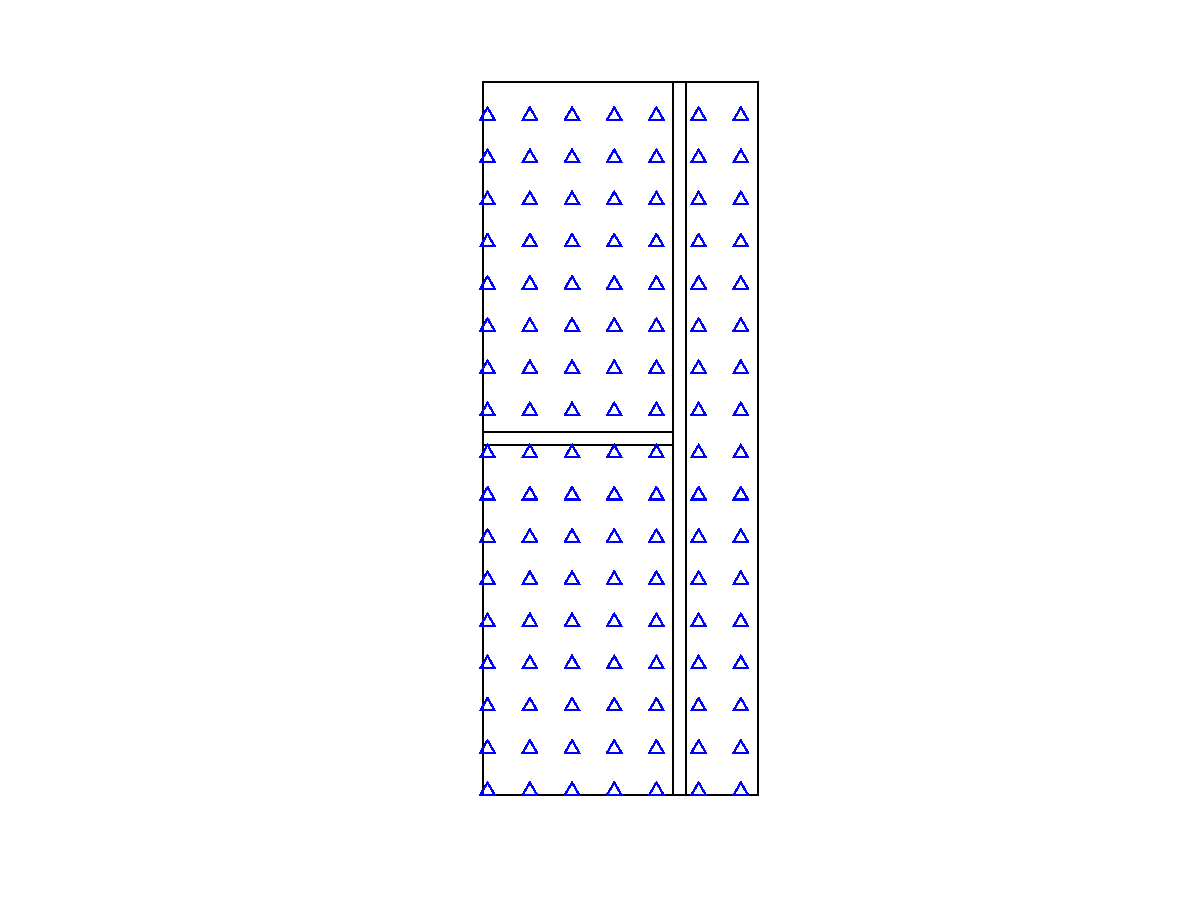
\includegraphics[width=3in]{map.eps}
\caption{Map}
\label{map}
\end{minipage}
\begin{minipage}[t]{0.5\linewidth}
\centering
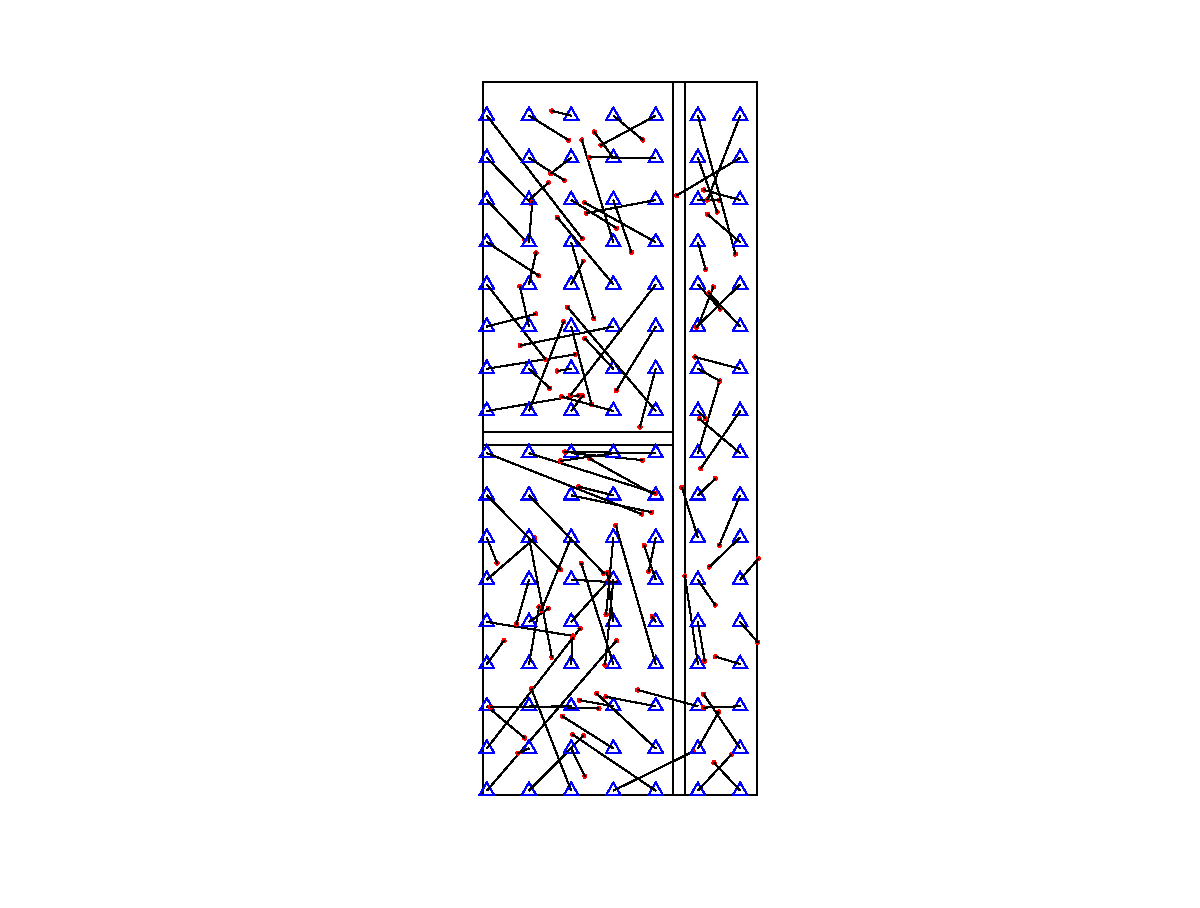
\includegraphics[width=3in]{SVR.eps}
\caption{SVM-regression}
\label{SVR}
\end{minipage}
\begin{minipage}[t]{0.5\linewidth}
\centering
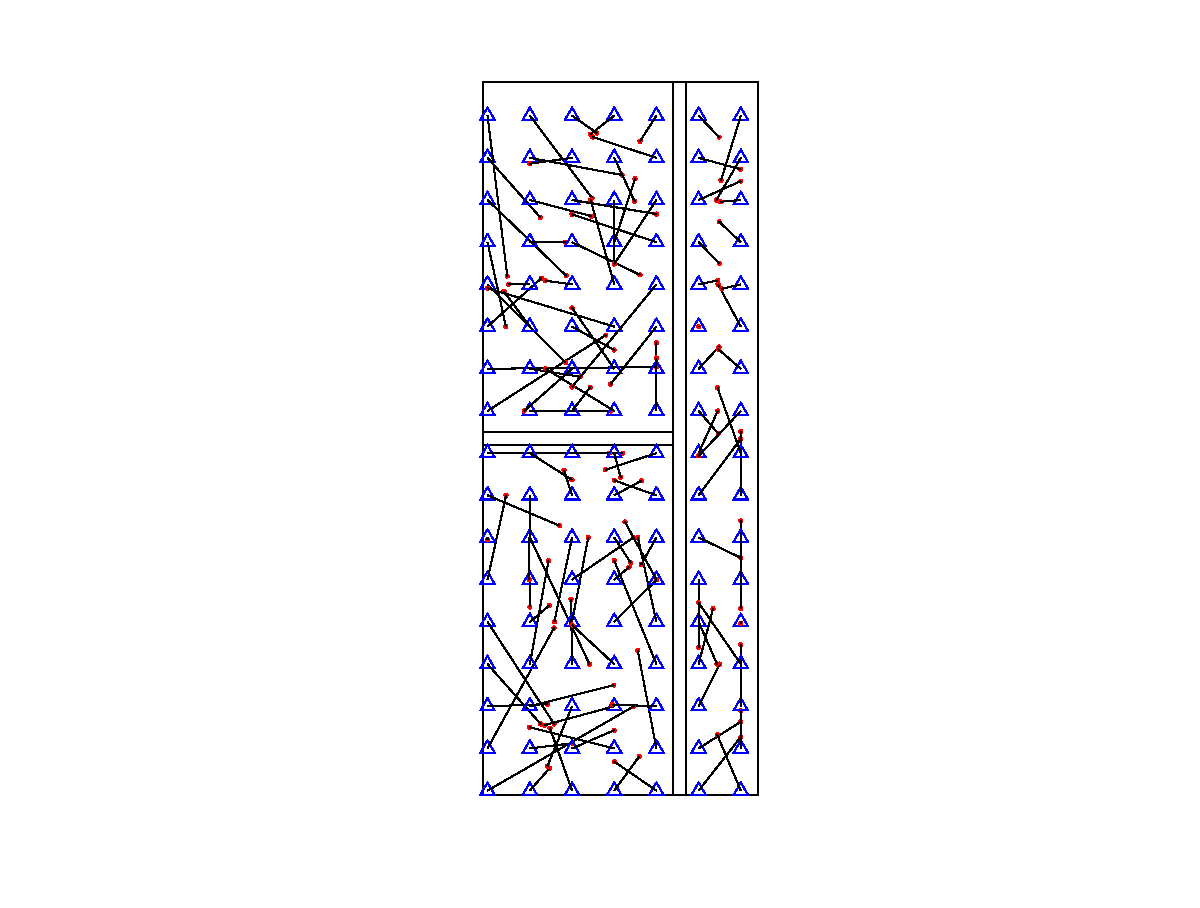
\includegraphics[width=3in]{WKNN.eps}
\caption{WKNN}
\label{WKNN}
\end{minipage}
\begin{minipage}[t]{0.5\linewidth}
\centering
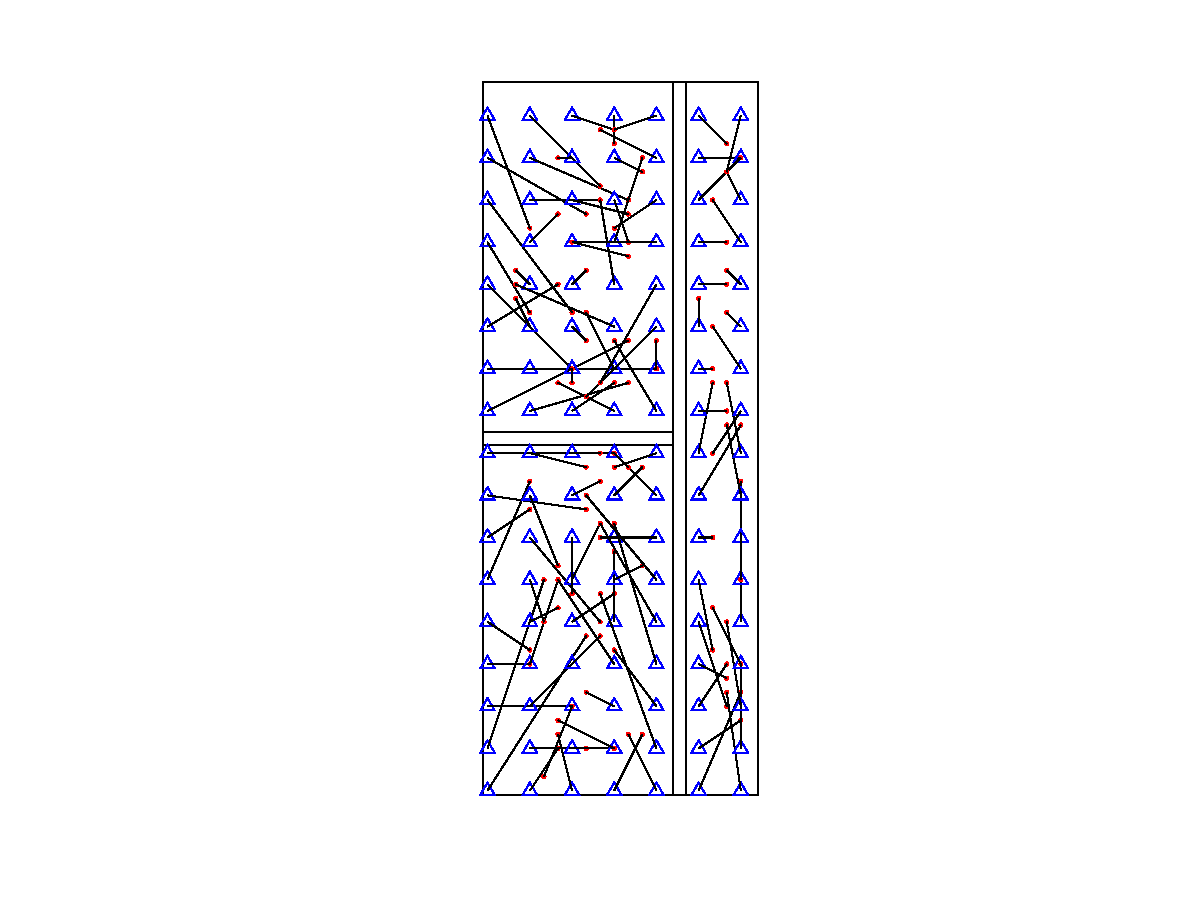
\includegraphics[width=3in]{KNN.eps}
\caption{KNN}
\label{KNN}
\end{minipage}
\end{figure}

三种方法中各点到其预测点的平均距离见下页表格,由表可见三种算法在leave-one-out实验中的平均误差都在1.5米左右。
\begin{table}[h]
\centering
\begin{tabular}{c|c}
Algorithm & Average distance\\\hline
SVM & 1.499\\
WKNN & 1.501\\
KNN & 1.568
\end{tabular}
\end{table}\\


\subsection{分类问题}
我们把地图分为112教室、111教室和走廊三类。以上三种回归算法自然也可以用来分类,此外我们也用SVM-classification算法(RBF kernel,$\gamma = 0.0001, C = 1$)进行了leave-one-out测试。除了SVM-regression算法有2个预测错误外(见图\eqref{SVR}),其他算法都没有错误。



\section{人员分工}
\begin{itemize}
 \item 胡威:位置预测算法的实现,服务器与数据库、服务器与客户端的部分接口。
 \item 李竺霖:客户端的部分界面设计(启动画面,按钮设计,整体布局,地图加载与位置标记的绘制),服务器与数据库、服务器与客户端的部分接口。
 \item 孔令航:客户端的Wifi扫描,与服务器的交互,部分界面设计(分栏设计与管理,整体布局,色带滑动的动画,进度条)。
\end{itemize}


\begin{thebibliography}{9}

\bibitem{1}
Martin, E., Vinyals, O., Friedland, G., and Bajcsy, R.
Precise Indoor Localization Using Smart Phones.
\emph{MM}, 2010.

\bibitem{2}
Chang, Chih-Chung and Lin, Chih-Jen.
LIBSVM: A library for support vector machines
Software available at \url{http://www.csie.ntu.edu.tw/~cjlin/libsvm}

\bibitem{3}
Christopher, M.
Pattern Recognition and Machine Learning.
\emph{Springer}, 2006.
\end{thebibliography}


\end{CJK*}



\end{document}
